% Template for ICASSP-2021 paper; to be used with:
%          spconf.sty  - ICASSP/ICIP LaTeX style file, and
%          IEEEbib.bst - IEEE bibliography style file.
% --------------------------------------------------------------------------
\documentclass{article}
\usepackage{spconf,amsmath,graphicx}

% Example definitions.
% --------------------
\def\x{{\mathbf x}}
\def\L{{\cal L}}

% Title.
% ------
\title{DIETARY INSIGHTS FROM SEAFOOD CONSUMPTION}
%
% Single address.
% ---------------
\name{Jorid Topi}
\address{Seafood Globalization Lab}
%
% For example:
% ------------
%\address{School\\
%	Department\\
%	Address}
%
% Two addresses (uncomment and modify for two-address case).
% ----------------------------------------------------------
%\twoauthors
%  {A. Author-one, B. Author-two\sthanks{Thanks to XYZ agency for funding.}}
%	{School A-B\\
%	Department A-B\\
%	Address A-B}
%  {C. Author-three, D. Author-four\sthanks{The fourth author performed the work
%	while at ...}}
%	{School C-D\\
%	Department C-D\\
%	Address C-D}
%
\begin{document}
%\ninept
%
\maketitle
%
\begin{abstract}
Using data from recent nutritional surveys, this project aims to explore whether seafood consumption is being driven by healthier choices from the consumer side. A machine learning modeling approach is used to contribute to the following research question, by analyzing a meal that contains seafood as a whole: Are food items that are consumed with seafood generally healthier than in meals where no seafood is present? The model is set up to classify a meal as a seafood meal or non-seafood meal, using the survey data to train the classifier. This classification model is then used to provide some explanation about the types of side dishes that are consumed by each group. Different types of modeling approaches are explored, attempting to find a model that best represents the population behavior.
\end{abstract}

\section{Introduction}
\label{sec:intro}

Global consumption of seafood has evolved in a rapid manner due in part to, technological advances in agriculture, lower costs in transportation, and a growth in consumer demand. The consumer demand may be driven by factors such as lower prices, more variety in the supply from growth in the global trade, or from evolving nutritional studies claiming that seafood is a healthier choice of protein source when compared to other types of meat. The National Health and Nutrition Examination Survey (NHANES), is an annual nutrition survey of the United States population designed and conducted by the National Center for Health Statistics. 

A machine learning classification model uses a combination of explanatory variables to predict, or classify, a categorical response variable. Recent advances in the field of machine learning provide a variety of classification modeling techniques, each with their own trade-offs in regards to the context of the dataset, or the problem it is attempting to address. In order to make a prediction of the response, classification models can use either (1) a linear combination of the explanatory variables (2) a non-linear combination of the explanatory variables (3) decision rules derived from the explanatory variables. 

By finding the best linear combination of the explanatory variables, the first approach provides a certain level of interpretability of the explanatory variables. In this context, the model aims to use the side dishes as explanatory variables, in order to predict whether the main choice of protein is seafood or meat. By interpreting the coefficients from the explanatory variables, inferences can be made about the characteristics of the side dishes that the two different groups are consuming. The second and third classification modeling approaches are also explored, in an attempt to uncover non-linear patterns about these side dish characteristics. 

\section{About the Dataset}
\label{sec:dataset}

\subsection{FPED Components}
\label{ssec:subhead}

The NHANES dataset contains survey information about the participants' food consumption over the last 24 hours. Each food item consumed is recorded as an individual observation that among other information, contains a textual description of the food item. The dataset that is used for this study contains an important transformation to this textual description. This transformation uses a set of standard dish recipes to break down each food item to quantitative nutritional components at the observation level. These nutritional components are defined in the Food Patterns Equivalents Database (FPED), and they provide a food item breakdown from a nutritional value perspective \cite{C2}. 

The main FPED components are Fruits, Vegetables, Grains, Dairy, Protein Foods, Added Sugars, Oils, Solid Fats, and Alcoholic Drinks. Apart from the last four components on this list, the rest are broken down to another level of detail, providing a quantity for the different types of the main components. For example, the Vegetables component is broken down to Tomatoes, Potatoes, and other vegetable types as defined in the FPED. The observations in the dataset are aggregated to provide meal level observations, adding the FPED component quantities for each food item within a meal. 

The figure below is a sample of the aggregated FPED components from a meal containing multiple food items, such as different types of sushi. This FPED distribution is very typical of meals within this dataset. The component makeup is sparse, i.e. only a few of the available components are present in this meal. Another important observation from this sample is the high quantity in the Oils component for this sushi meal. It is evident that the Oils component is derived from the seafood items themselves, which are meant to be isolated as the dependent variable in this study.

\begin{figure}[htb]
\begin{minipage}[b]{.48\linewidth}
  \centering
  \centerline{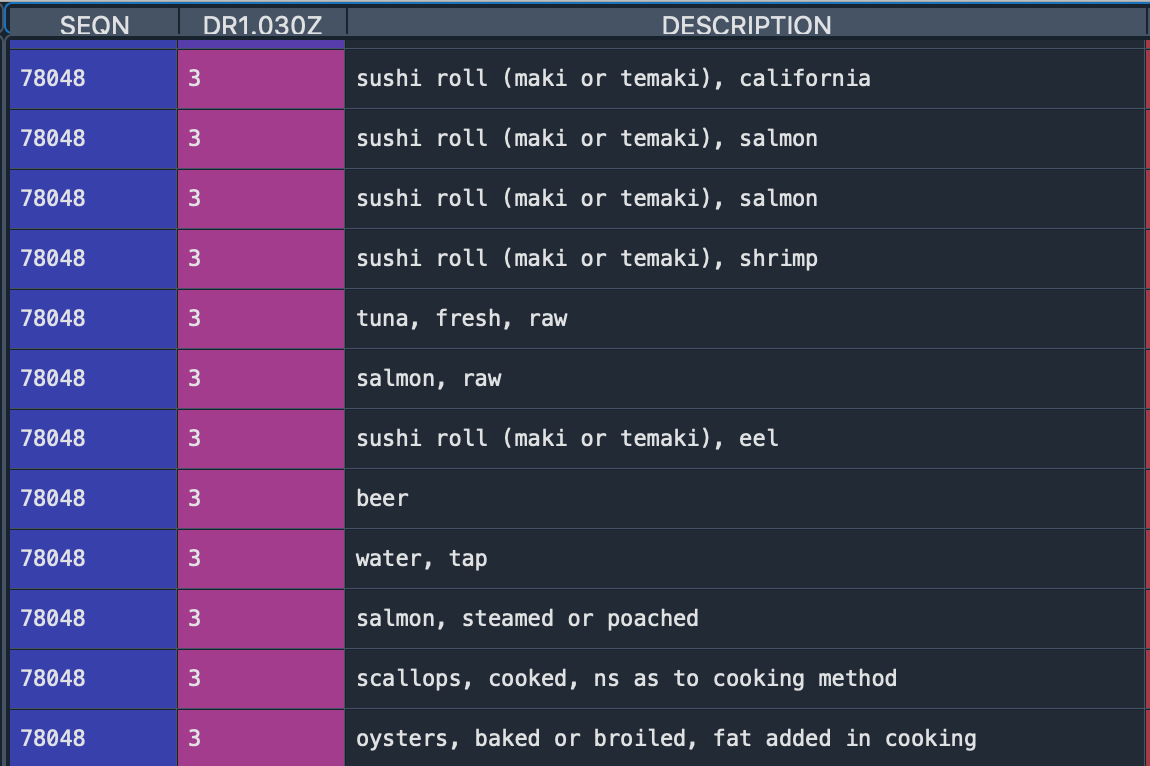
\includegraphics[scale=0.175]{sushi_meal_desc.png}}
  \centerline{(a) Dataset Meal Sample}\medskip
\end{minipage}
\hfill
\begin{minipage}[b]{0.48\linewidth}
  \centering
  \centerline{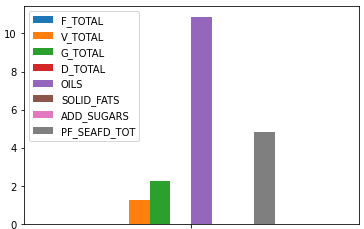
\includegraphics[scale=0.3]{sushi_meal.png}}
  \centerline{(b) Sample FPED Components}\medskip
\end{minipage}
\caption{Example of Data Transformation}
\label{fig:res}
\end{figure}

\subsection{Data Pre-Processing}
\label{ssec:subhead}

As previously mentioned, the NHANES dataset is very complex in terms of the survey design. As such, a special focus is necessary in order to obtain an observation space that is best suited for studying the research question at hand. The following logic has been applied to the dataset in order to obtain this desired observation space:

\subsubsection{Meal Selection}
\label{sssec:subsubhead}

Only meals that are either lunch or dinner are selected from the dataset. This is due to these meals being the most likely to contain seafood as a choice. Meals such as breakfast and snacks are excluded for this reason. Vegetarian meals are excluded from the final observation space, since consumers that identify as vegetarian are not a subject for this study. Since a variable for participants who identify themselves as vegetarian does not exist, any meal that does not contain seafood or meat is dropped.

\subsubsection{Seafood Meal Classification}
\label{sssec:subsubhead}

A meal is classified as seafood or non-seafood based on the Protein Foods FPED component content for seafood or meat. The dataset contains meals where both seafood and meat are present, making these meals ambiguous in terms of the classification. A seafood to meat quantity ratio is used to classify the meal. Meals with ratios that are in a middle range are dropped from the dataset, due to the ambiguity on whether the consumer choice was specifically seafood or meat. 

\subsubsection{Demographic Selection}
\label{sssec:subsubhead}

Since they are the most likely to make their own individual choices regarding side dishes, only participants that are 18 of age or older are selected for the study. In addition to this, only meals that are consumed at home are selected. This is due to the fact that side dishes for restaurant meals are restricted from a pre-set menu.

\section{Logistic Regression}
\label{sec:pagestyle}

\subsection{Model Setup}
\label{ssec:subhead}

A logistic regression is used to provide a classification among two classes, using a linear combination of the explanatory variables. A meal is classified as either (1) Seafood Meal or (2) Non-seafood Meal using the Protein Food FPED component breakdown for seafood and meat. The model uses the FPED components at the lowest available level, excluding the Protein Foods components for seafood and meats. This comes out to a total of 22 independent variables. The prediction of the probability is then given by the following equation:\\

$\hat{Pr}(meal = seafood | X) = \frac{e^{\beta_0 + \beta_1X_1 + ... + \beta_pX_{22}}}{1 + e^{\beta_0 + \beta_1X_1 + ... + \beta_pX_{22}}}$\\

Where X represents the 22 independent variables. In this setup, if $\hat{Pr} > 0.5$, then the prediction outcome is a seafood meal. Otherwise, the prediction outcome is a non-seafood meal. 

\subsection{Model Evaluation}
\label{ssec:subhead}

In order to account for an imbalance in the observation count among the two classes, the input to the model is equally sampled at $N = 1000$ for each class. The data is then split to: 80\% or $N=800$ per class, to train the model and 20\% or $N=200$ per class, to test the model. A prediction accuracy score is generated for both the training and test data. For the training data, this score indicates how good the model is at fitting to the training data. For the test data, this score indicates the goodness of fit of the model, or how well the model can predict the real world data. In order to account for the random sampling of the input data, the model is evaluated 100 times with 100 different samples. The distribution of the prediction scores over these 100 runs for both the training and test data is provided below:\\

\begin{figure}[htb]
\begin{minipage}[b]{.48\linewidth}
  \centering
  \centerline{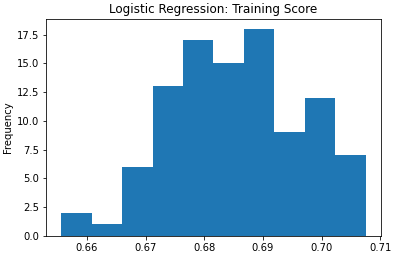
\includegraphics[scale=0.3]{Log_Reg_Train_Score.png}}
\end{minipage}
\hfill
\begin{minipage}[b]{0.48\linewidth}
  \centering
  \centerline{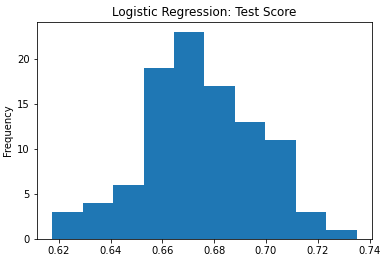
\includegraphics[scale=0.3]{Log_Reg_Test_Score.png}}
\end{minipage}
\caption{Distribution of Accuracy Scores Over 100 Runs}
\label{fig:res}
\end{figure}

These results show that the model is equally good at fitting the training data and predicting on the test set. The prediction score for each instance is concentrated in the 66\% to 70\% range over the 100 runs.

\subsection{Model Interpretation}
\label{ssec:subhead}

\subsubsection{Regression Coefficients}
\label{sssec:subsubhead}

The regression coefficients for the logistic regression model are estimated using the maximum likelihood method. The most basic form of interpretation of the coefficient is by using their sign to determine how the associated parameter affects the probability $p(X)$. While holding the other parameters constant: (1) If the coefficient is positive, then increasing the associated parameter will increase the probability of a seafood meal, while decreasing the associated parameter has the opposite effect. (2) The inverse of this interpretation logic is true if the sign of the coefficient is negative.

Due to the exponents and non-linear nature of the logistic equation, the magnitude of the coefficients requires a non-linear transformation in order to be interpreted. This form of interpretation of the logistic regression coefficients is called the log odds ratio. This is since the logistic regression function can be simplified to the linear parameter combination form, which is equal to the log of the odds ratio as follows:\\

$log(\frac{p(X)}{1 - p(X)}) = \beta_0 + \beta_1X_1 + ... + \beta_{22}X_{22}$\\

While holding the other parameters constant: (1) Increasing a parameter by one unit will change the log odds ratio by the magnitude of the associated coefficient. (2) Decreasing a parameter by one unit will change the log odds ratio by the negative magnitude of the associated coefficient. 

\subsubsection{Coefficient Test Scores}
\label{sssec:subsubhead}

In a regression model, the null hypothesis for the parameter estimation is as follows:\\

$H_0: \beta_i = 0$\\

In other words, the null hypothesis states that in the real population, the parameter does not provide any contribution to the classification of a seafood meal using logistic regression. The derived p-value for each coefficient estimation provides the metric that supports or rejects this null hypothesis. The p-values associated with each parameter coefficient were averaged over the 100 training runs, and the parameters with the most significant p-values are listed in the table below.\\

\begin{figure}[htb]
\begin{minipage}[b]{.48\linewidth}
  \centering
  \centerline{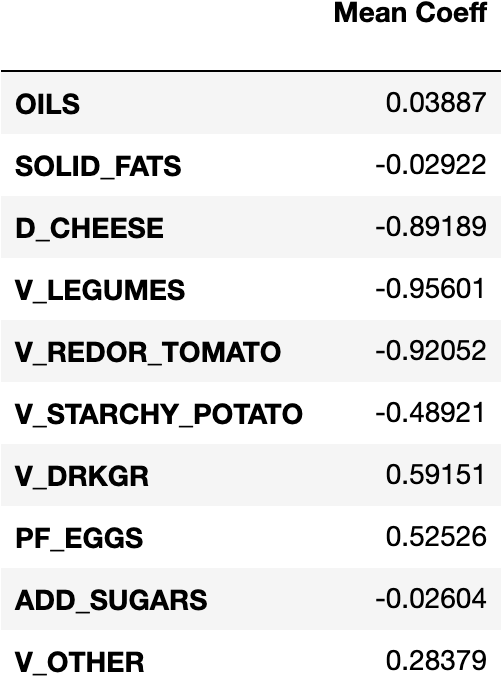
\includegraphics[scale=0.3]{Coeff_Values_Top10.png}}
\end{minipage}
\hfill
\begin{minipage}[b]{0.48\linewidth}
  \centering
  \centerline{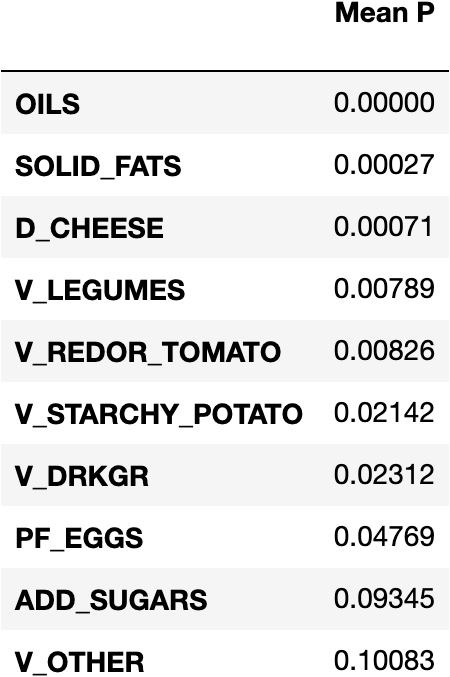
\includegraphics[scale=0.3]{P_Value_Means_Top10.png}}
\end{minipage}
\caption{Mean Coefficient and P-Values of Most Significant Components From 100 Runs}
\label{fig:res}
\end{figure}

The components for Oils and Solid Fats are the most significant on average. It is likely that this is due to these components being part of seafood and meat items, indicating a correlation with the response. Unlike the Protein Foods components that are strictly associated with seafood and meats, Oils and Solid Fats cannot be isolated from the response, due to the fact that they may also be part of the side dishes themselves.

The coefficient estimate distribution over the 100 runs is displayed in the plots below for the components with the 10 most significant values, and for the components with the 10 least significant values:\\

\begin{figure}[htb]
\begin{minipage}[b]{.48\linewidth}
  \centering
  \centerline{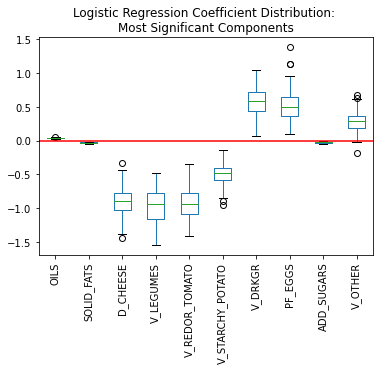
\includegraphics[scale=0.3]{Coeff_Est_Top10_P.png}}
\end{minipage}
\hfill
\begin{minipage}[b]{0.48\linewidth}
  \centering
  \centerline{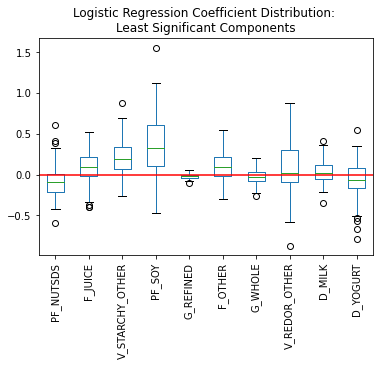
\includegraphics[scale=0.3]{Coeff_Est_Tail10_P.png}}
\end{minipage}
\caption{Distribution of Regression Coefficients Over 100 Runs}
\label{fig:res}
\end{figure}

The coefficient estimates for the components with the 10 most significant values have a more stable sign over the 100 runs, providing a more clear indication of how these parameters contribute to the probability of a meal containing seafood. The coefficient estimates for the components with the 10 least significant values have a more unstable sign over the 100 runs, proving to be unreliable when determining their contribution to the response. 

\subsection{Model Diagnostics}
\label{ssec:subhead}

This section looks at potential issues with the logistic model approach with this particular dataset. Unique characteristics of the data are explored, as well as potential issues with the high number of independent variables that are used to fit the regression model. This is in response to the model accuracy score on the training data, which indicates that the model is not fitting the training data very well.

\subsubsection{Component Characteristics}
\label{sssec:subsubhead}

The plots below are showing the distributions of two significant FPED components among the two groups of the response variable. 

\begin{figure}[htb]
\begin{minipage}[b]{.48\linewidth}
  \centering
  \centerline{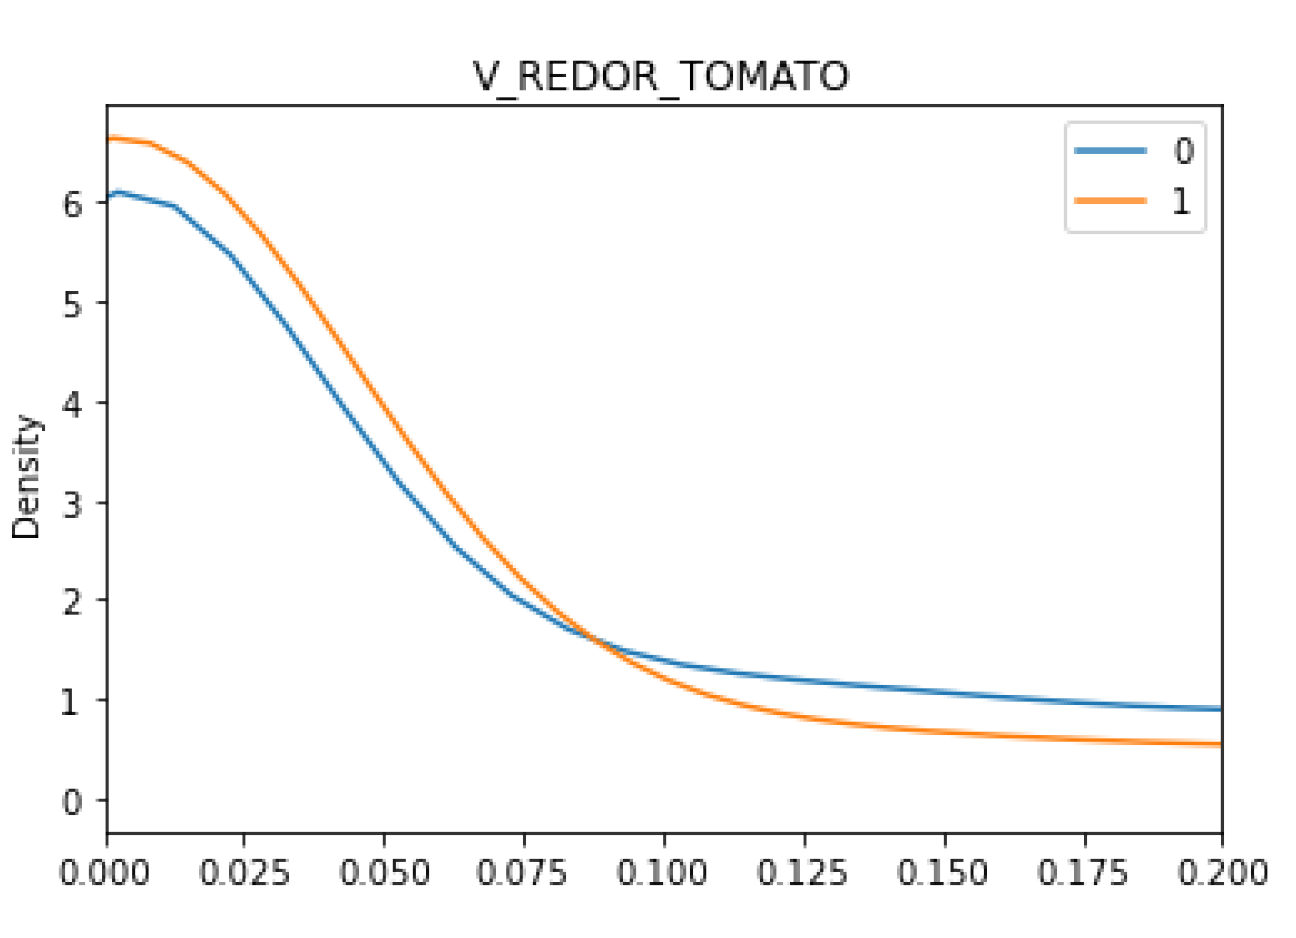
\includegraphics[scale=0.175]{V_REDOR_TOMATO_kde.png}}
\end{minipage}
\hfill
\begin{minipage}[b]{0.48\linewidth}
  \centering
  \centerline{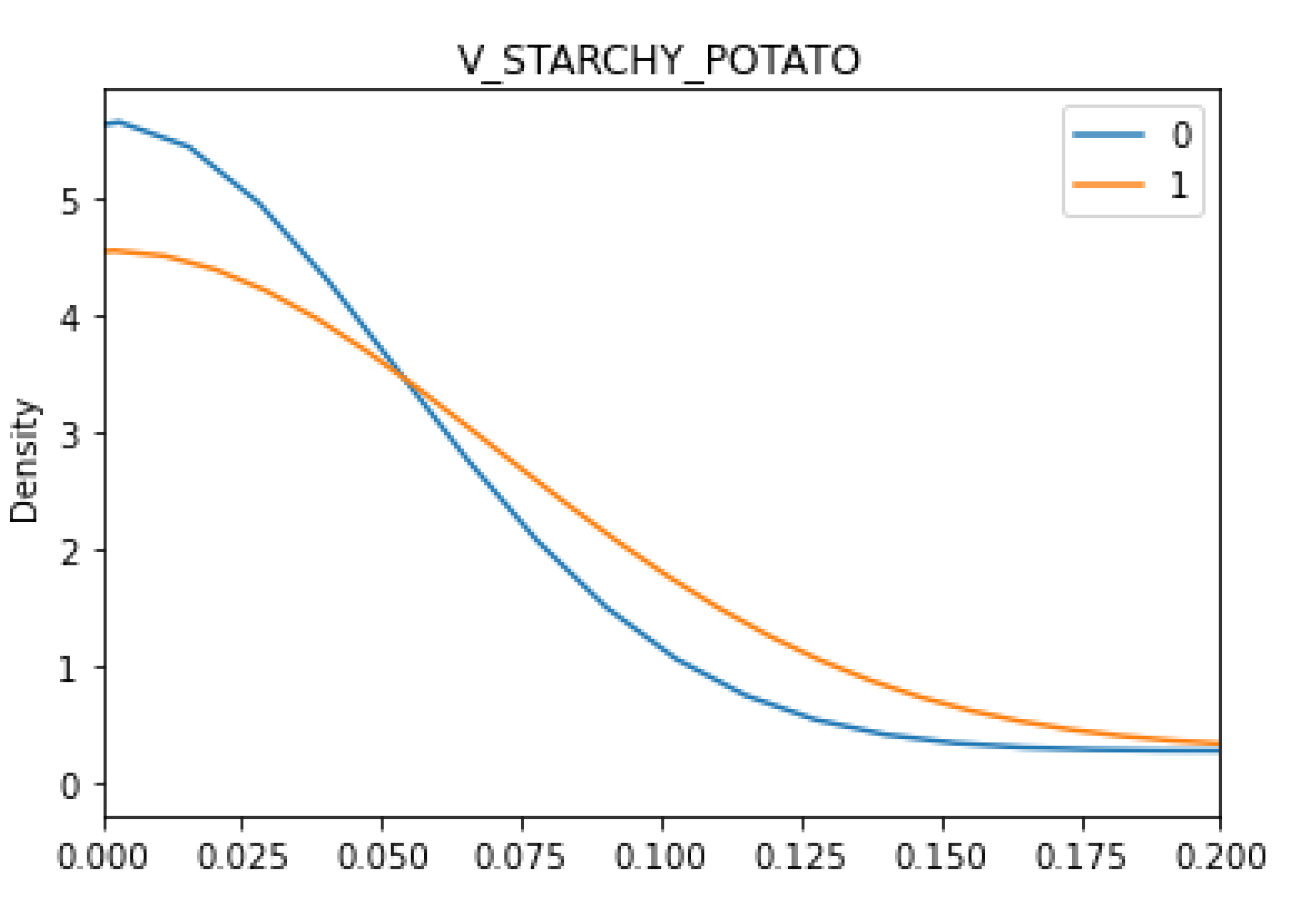
\includegraphics[scale=0.175]{V_STARCHY_POTATO_kde.png}}
\end{minipage}
\caption{Example of Component Density Plot}
\label{fig:res}
\end{figure}

\begin{figure}[htb]
\begin{minipage}[b]{.48\linewidth}
  \centering
  \centerline{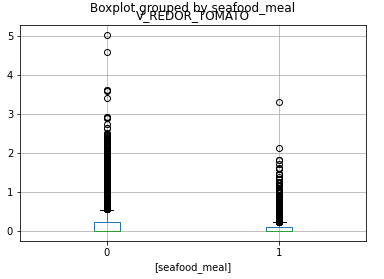
\includegraphics[scale=0.3]{V_REDOR_TOMATO_box_plot.png}}
\end{minipage}
\hfill
\begin{minipage}[b]{0.48\linewidth}
  \centering
  \centerline{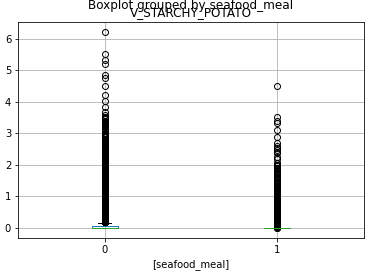
\includegraphics[scale=0.3]{V_STARCHY_POTATO_box_plot.png}}
\end{minipage}
\caption{Example of Component Box Plot}
\label{fig:res}
\end{figure}

Two main characteristics are evident from these independent variables: (1) From the density plot, we can see that there is a high number of 0 values in the data, i.e. the data is very sparse. This was also apparent in the sushi meal example discussed in a previous section. Any one meal will not typically contain all the FPED components, but rather a subset of them at any one time. (2) These components contain many outliers, so the data distribution has a long right tail. The high number of outliers is evident from the boxplots above.

Similar plots and statistics were generated for all the FPED components among the two groups. While only a sample of two components is shown above, all the FPED components follow a similar pattern in terms of statistical distribution. From the density plots, it seems evident that there is not a very distinct separation of these components among the two classes. This may be a reason for the training accuracy score of the model rarely reaching above 70\% prediction accuracy. 

\subsubsection{Dimensionality}
\label{sssec:subsubhead}

The logistic regression model can be susceptible to issues with multicollinearity among the independent variables. Since this model is trained with 22 independent variables, the potential for multicollinearity and other issues related to the high dimensions demands some exploration. The figure below is showing a heat map of the correlation matrix among the 22 FPED components:\\

\begin{figure}[htb]
\begin{minipage}[b]{1.0\linewidth}
  \centering
  \centerline{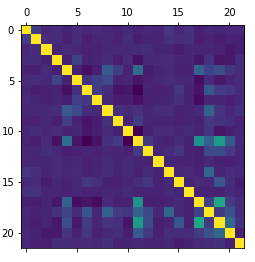
\includegraphics[scale=0.35]{Corr_Matrix.png}}
\end{minipage}
\caption{FPED Component Correlation Matrix}
\label{fig:res}
\end{figure}

The heatmap is not showing any issues with correlation among the independent variables. In order to further rule out issues with dimensionality, a PCA analysis was used on the observation space. The logistic regression model was then fitted and evaluated using the first 5 principal components that were generated from the analysis.\\

\begin{figure}[htb]
\begin{minipage}[b]{.48\linewidth}
  \centering
  \centerline{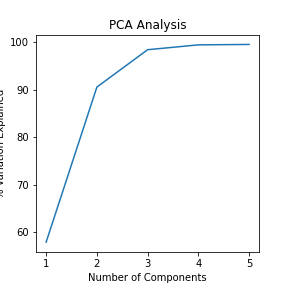
\includegraphics[scale=0.4]{PCA_Analysis.png}}
\end{minipage}
\hfill
\begin{minipage}[b]{0.48\linewidth}
  \centering
  \centerline{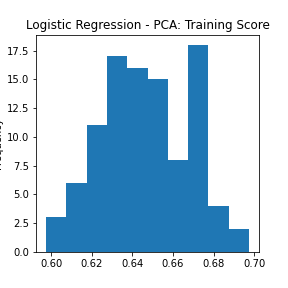
\includegraphics[scale=0.4]{Log_Reg_PCA_Training_Score.png}}
\end{minipage}
\caption{PCA Analysis and Model Performance}
\label{fig:res}
\end{figure}

The plots are showing that the first 5 principal components are explaining almost all of the variation in the data. The training accuracy score of the model that is fitted with these 5 principal components is actually a bit poorer than the baseline model that includes all the FPED components. This is further indication that dimensionality does not appear to be an issue with the baseline model.

\section{Non-Parametric Models}
\label{sec:pagestyle}

Non-parametric models are more flexible with fitting to the training data than parametric ones, such as the logistic regression model. This is because they are particularly good at finding non-linear patterns in the data, so a few popular non-parametric models were explored in an attempt to find such patterns among the FPED components. 
\subsection{Support Vector Machine}
\label{ssec:subhead}

A simple Support Vector Machine classifier was fitted in a similar setup to the baseline models. These are the results over 100 training runs:\\

\begin{figure}[htb]
\begin{minipage}[b]{.48\linewidth}
  \centering
  \centerline{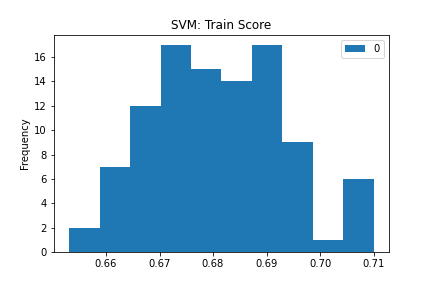
\includegraphics[scale=0.3]{SVM_Train_Score.png}}
\end{minipage}
\hfill
\begin{minipage}[b]{0.48\linewidth}
  \centering
  \centerline{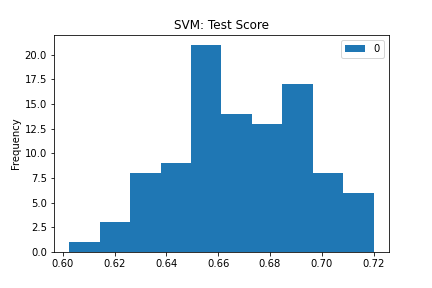
\includegraphics[scale=0.3]{SVM_Test_Score.png}}
\end{minipage}
\caption{SVM Model Evaluation}
\label{fig:res}
\end{figure}

The linear SVM model does not provide any improvement from the baseline logistic regression model. A kernel SVM approach could be explored to provide more flexibility to the fit.

\subsection{Decision Tree}
\label{ssec:subhead}

Decision trees derive logical branches that are fitted to the independent variables in order to, in this case, classify the meal. One unique advantage to decision trees is the explanatory power of the logical branches. These are the results of a decision tree fit over 100 runs:\\

\begin{figure}[htb]
\begin{minipage}[b]{.48\linewidth}
  \centering
  \centerline{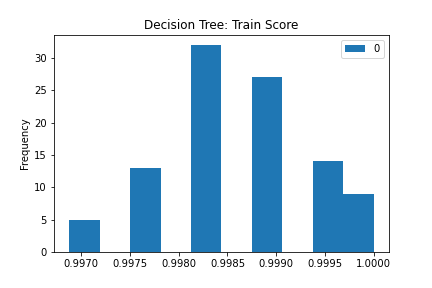
\includegraphics[scale=0.3]{Tree_Train_Score.png}}
\end{minipage}
\hfill
\begin{minipage}[b]{0.48\linewidth}
  \centering
  \centerline{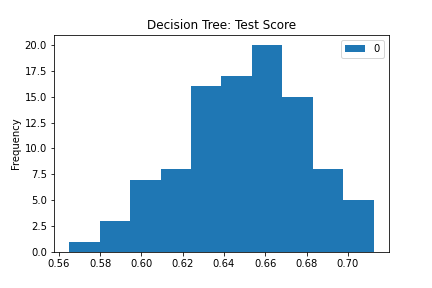
\includegraphics[scale=0.3]{Tree_Test_Score.png}}
\end{minipage}
\caption{Decision Tree Evaluation}
\label{fig:res}
\end{figure}

The decision tree produces a very high accuracy score on the training set, indicating that the model is very good at fitting to the data. However, the performance over the test set does not provide a lot of improvement from the other models, indicating that the training data is overfitted. 

\subsection{Simple Neural Network}
\label{ssec:subhead}

Using deep learning methods, neural networks are particularly good at finding non-linear patterns in the data. A simple neural network was explored, using 7 hidden layers and up to 1000 epochs of training. A plot of the training history is shown below:\\

\begin{figure}[htb]
\begin{minipage}[b]{1.0\linewidth}
  \centering
  \centerline{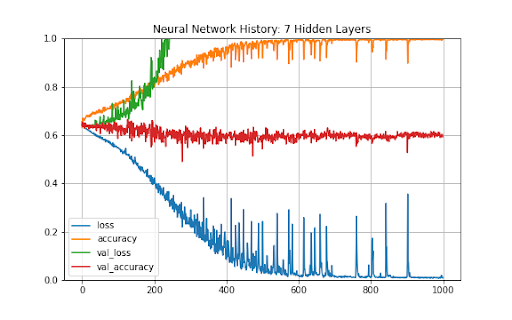
\includegraphics[scale=0.4]{Neural_Network_History.png}}
\end{minipage}
\caption{Neural Network Training History}
\label{fig:res}
\end{figure}

The training accuracy score starts to reach 100\% at around 650 epochs of training, so this model is also really good at fitting the training data. However, the accuracy score on the test data is constantly at around 60\%. Similar to the decision tree, the model is overfitting the training data, but those same patterns do not apply to the test set.

\section{Conclusions}
\label{sec:pagestyle}

\subsection{Final Remarks}
\label{ssec:subhead}

A high accuracy score on the test data is important for providing an acceptable level of confidence that the model represents the behavior of the real world population. Since the models that were explored in this project do not provide very high accuracy scores on the test data, it is possible that a behavioral pattern does not exist between seafood and non-seafood consumers. If this pattern does exist, it may be the case that it is not properly modeled using the FPED components. For example, the FPED components cannot completely isolate the side dishes (independent variables) from the seafood or meat items (dependent variables). This was evident from the Oils and Solid Fats components being the most significant contributors to the logistic regression model, where both components are also part of seafood and meat items. 

\subsection{Forward Work}
\label{ssec:subhead}

Due to the complex nature of the survey data that was studied in this project, there are numerous possibilities for deriving insights about seafood consumers. Such possibilities exist in the consumer demographics, seafood cooking methods, and seafood species consumption. Another avenue for analysis exists in the textual description of the food items, as an alternative to the FPED component approach. A textual analysis can be performed on different clusters of meals, where clusters can be derived by (1) class separation of seafood vs non-seafood meals, or seafood species (2) an unsupervised learning approach. 


% To start a new column (but not a new page) and help balance the last-page
% column length use \vfill\pagebreak.
% -------------------------------------------------------------------------
%\vfill
%\pagebreak

\vfill\pagebreak

% References should be produced using the bibtex program from suitable
% BiBTeX files (here: strings, refs, manuals). The IEEEbib.bst bibliography
% style file from IEEE produces unsorted bibliography list.
% -------------------------------------------------------------------------
\bibliographystyle{IEEEbib}
\bibliography{test}

\end{document}
